\documentclass{article} % For LaTeX2e
\usepackage{final_project,times,graphicx}
%\documentstyle[nips12submit_09,times,art10]{article} % For LaTeX 2.09


\title{Predicting the Impact of Research Papers in the Covid-19 Open Research Dataset}



\author{
Tyler Ashoff \\
Department of Interdisciplinary Data Science\\
Duke University\\
Durham, NC 27708 \\
\texttt{tyler.ashoff@duke.edu} \\
\\
\textbf{Jennifer Wilson} \\
Department of Statistical Science\\
Duke University\\
Durham, NC 27708 \\
\texttt{jennifer.wilson994@duke.edu} \\
}

\newcommand{\fix}{\marginpar{FIX}}
\newcommand{\new}{\marginpar{NEW}}

\nipsfinalcopy

\begin{document}


\maketitle

Abstract

\begin{abstract}
The volume of research papers  and articles relating to Coronaviruses combined with the rapid increase at which new information is being published makes it nearly impossible for those relying on this research to keep up [1]. We propose the use of citation count prediction [2] to identify impactful articles which may have been overlooked.
\end{abstract}

\section{Final papers for STA613/CBB540, 2013}

Please read carefully the
instructions below, and follow them faithfully.
\subsection{Style}

Papers describing final project should be up to four pages long (not including bibliography). They should contain an abstract, introduction, related work, methods, results, discussion, and conclusion section, and figures and tables where necessary, and a bibliography. These papers are due on April 16th in class.


\subsection{Retrieval of style files}

The formatting instructions contained in these style files are summarized in


\section{General formatting instructions}
\label{gen_inst}

The text must be confined within a rectangle 5.5~inches (33~picas) wide and
9~inches (54~picas) long. The left margin is 1.5~inch (9~picas).
Use 10~point type with a vertical spacing of 11~points. Times New Roman is the
preferred typeface throughout. Paragraphs are separated by 1/2~line space,
with no indentation.

Paper title is 17~point, initial caps/lower case, bold, centered between
2~horizontal rules. Top rule is 4~points thick and bottom rule is 1~point
thick. Allow 1/4~inch space above and below title to rules. All pages should
start at 1~inch (6~picas) from the top of the page.


\section{Headings: first level}
\label{headings}

First level headings are lower case (except for first word and proper nouns),
flush left, bold and in point size 12. One line space before the first level
heading and 1/2~line space after the first level heading.

\subsection{Headings: second level}

Second level headings are lower case (except for first word and proper nouns),
flush left, bold and in point size 10. One line space before the second level
heading and 1/2~line space after the second level heading.

\subsubsection{Headings: third level}

Third level headings are lower case (except for first word and proper nouns),
flush left, bold and in point size 10. One line space before the third level
heading and 1/2~line space after the third level heading.

\section{Citations, figures, tables, references}
\label{others}

These instructions apply to everyone, regardless of the formatter being used.

\subsection{Citations within the text}

Citations within the text should be numbered consecutively. The corresponding
number is to appear enclosed in square brackets, such as [1] or [2]-[5]. The
corresponding references are to be listed in the same order at the end of the
paper, in the \textbf{References} section. (Note: the standard
\textsc{Bib\TeX} style \texttt{unsrt} produces this.) As to the format of the
references themselves, any style is acceptable as long as it is used
consistently.

\subsection{Figures}

All artwork must be neat, clean, and legible. Lines should be dark
enough for purposes of reproduction; art work should not be
hand-drawn. The figure number and caption always appear after the
figure. Place one line space before the figure caption, and one line
space after the figure. The figure caption is lower case (except for
first word and proper nouns); figures are numbered consecutively.

Make sure the figure caption does not get separated from the figure.
Leave sufficient space to avoid splitting the figure and figure caption.


\begin{figure}[h]
\begin{center}
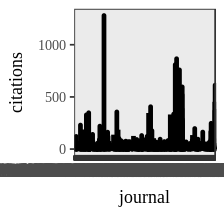
\includegraphics[scale=0.5]{../Figures/test1.png} 
\end{center}
\caption{Sample ggplot}
\end{figure}


\subsection{Tables}

All tables must be centered, neat, clean and legible. Do not use hand-drawn
tables. The table number and title always appear before the table. See


Place one line space before the table title, one line space after the table
title, and one line space after the table. The table title must be lower case
(except for first word and proper nouns); tables are numbered consecutively.


% latex table generated in R 3.5.3 by xtable 1.8-3 package
% Thu Apr 30 17:33:30 2020
\begin{table}[ht]
\centering
\caption{Xtable Example} 
\begin{tabular}{rllllllllllllllllllll}
  \hline
 &       X1 &   cord\_uid &     sha &   source\_x &    title &     doi &    pmcid &   pubmed\_id &   license &   abstract & publish\_time &   authors &   journal & Microsoft Academic Paper ID & WHO \#Covidence & has\_pdf\_parse & has\_pmc\_xml\_parse & full\_text\_file &     url &   citations \\ 
  \hline
X & Min.   :    0   & Length:22969       & Length:22969       & Length:22969       & Length:22969       & Length:22969       & Length:22969       & Min.   :    2142   & Length:22969       & Length:22969       & Length:22969       & Length:22969       & Length:22969       & Mode:logical   & Mode:logical   & Mode :logical   & Mode :logical   & Length:22969       & Length:22969       & Min.   :   0.00   \\ 
  X.1 & 1st Qu.: 5972   & Class :character   & Class :character   & Class :character   & Class :character   & Class :character   & Class :character   & 1st Qu.:19086376   & Class :character   & Class :character   & Class :character   & Class :character   & Class :character   & NA's:22969     & NA's:22969     & FALSE:4827      & FALSE:3985      & Class :character   & Class :character   & 1st Qu.:   0.00   \\ 
  X.2 & Median :11911   & Mode  :character   & Mode  :character   & Mode  :character   & Mode  :character   & Mode  :character   & Mode  :character   & Median :25089808   & Mode  :character   & Mode  :character   & Mode  :character   & Mode  :character   & Mode  :character   &  &  & TRUE :18142     & TRUE :18984     & Mode  :character   & Mode  :character   & Median :   4.00   \\ 
  X.3 & Mean   :14911   &  &  &  &  &  &  & Mean   :23086865   &  &  &  &  &  &  &  &  &  &  &  & Mean   :  12.94   \\ 
  X.4 & 3rd Qu.:23306   &  &  &  &  &  &  & 3rd Qu.:29111237   &  &  &  &  &  &  &  &  &  &  &  & 3rd Qu.:  13.00   \\ 
  X.5 & Max.   :52392   &  &  &  &  &  &  & Max.   :32277299   &  &  &  &  &  &  &  &  &  &  &  & Max.   :1280.00   \\ 
  X.6 &  &  &  &  &  &  &  & NA's   :2973   &  &  &  &  &  &  &  &  &  &  &  &  \\ 
   \hline
\end{tabular}
\end{table}




\section{Final instructions}
Do not change any aspects of the formatting parameters in the style
files.  In particular, do not modify the width or length of the
rectangle the text should fit into, and do not change font sizes.
Please note that pages should be numbered.

\section{Preparing PostScript or PDF files}

Please prepare PostScript or PDF files with paper size ``US Letter'', and
not, for example, ``A4''. The -t
letter option on dvips will produce US Letter files.

\begin{itemize}

\item Consider directly generating PDF files using \verb+pdflatex+

\item Otherwise, please generate your PostScript and PDF files with the following commands:
\begin{verbatim} 
dvips mypaper.dvi -t letter -Ppdf -G0 -o mypaper.ps
ps2pdf mypaper.ps mypaper.pdf
\end{verbatim}
\end{itemize}


\subsubsection*{Acknowledgments}

Use unnumbered third level headings for the acknowledgments. All
acknowledgments go at the end of the paper.

\subsubsection*{References}

References follow the acknowledgments. Use unnumbered third level heading for
the references. Any choice of citation style is acceptable as long as you are
consistent. CITE A LOT. Any unreferenced methods, prior work, or biological phenomenon, unless it is textbook-common, will be penalized.

\small{
[1] Allen Institute For AI. “COVID-19 Open Research Dataset Challenge (CORD-19).” Kaggle, CDC, 25 Apr. 2020, www.kaggle.com/allen-institute-for-ai/CORD-19-research-challenge.

[2] Yan, Rui \& Tang, Jie \& Liu, Xiaobing \& Shan, Dongdong \& Li, Xiaoming. (2011). Citation count prediction: Learning to estimate future citations for literature. {\itInternational Conference on  Information and Knowledge Management, Proceedings} 1247-1252. 10.1145/2063576.2063757. 
}


\end{document}
